
\subsubsection[Distribution-based (GMM)]{Distribution-based \textit{(GMM)}}
\begin{frame}

	\frametitle{{\color{GradientDescentDiagramOrange}Distribution-based Clustering}, in sintesi}

	%\begin{block}{}
		Il distribution-based clustering presuppone che i dati siano composti da distribuzioni, come le distribuzioni gaussiane.
		\newlinedouble
		Nella figura, il distribution-based clustering clusterizza i dati in tre distribuzioni gaussiane.
		All'aumentare della distanza dal centro della distribuzione, la probabilità che un punto appartenga alla distribuzione diminuisce.\\
		Le bande mostrano che la probabilità diminuisce. Se non conosci il tipo di distribuzione nei tuoi dati, dovresti usare un algoritmo diverso.
		\begin{figure}[!htbp]
			\centering
			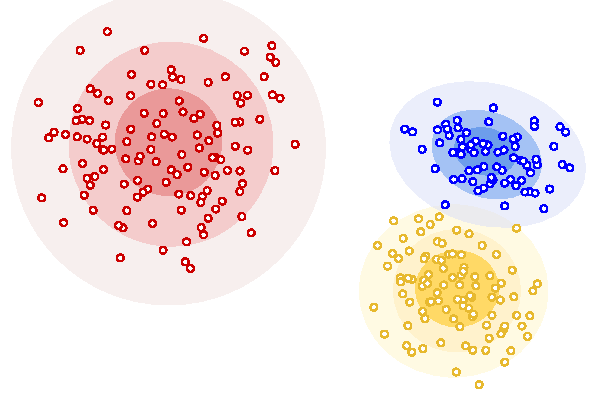
\includegraphics[width=5.0cm]{images/unsupervised/types/Clustering_Distribution.pdf}
					%\caption{Stripe Radar for Fraud Detection}
		\end{figure}
	%\end{block}

\end{frame}


\begin{frame}

	\frametitle{{\color{GradientDescentDiagramOrange}Distribution-based Clustering}: Mixture of Gaussian}

		\begin{columns}

			\column{0.55\linewidth}
			\begin{itemize}
				\item con il clustering K-means, la forma dei cluster è sempre la stessa: sferica attorno al centro del cluster
				\item una soluzione più flessibile è consentire alla forma di ciascun cluster di conformarsi a una gaussiana multivariata
				\item la distribuzione dei dati è modellata da una mistura di distribuzioni gaussiane (\textbf{mixture of Gaussian}), ogni cluster corrispondente a un componente della mistura
					\begin{itemize}
						\item[--] ogni cluster è caratterizzato non solo da una media $\mu_k$, ma anche da una matrice di covarianza $C_k$
					\end{itemize}
			\end{itemize}

			\column{0.45\linewidth}
			\begin{figure}[!htbp]
				\centering
				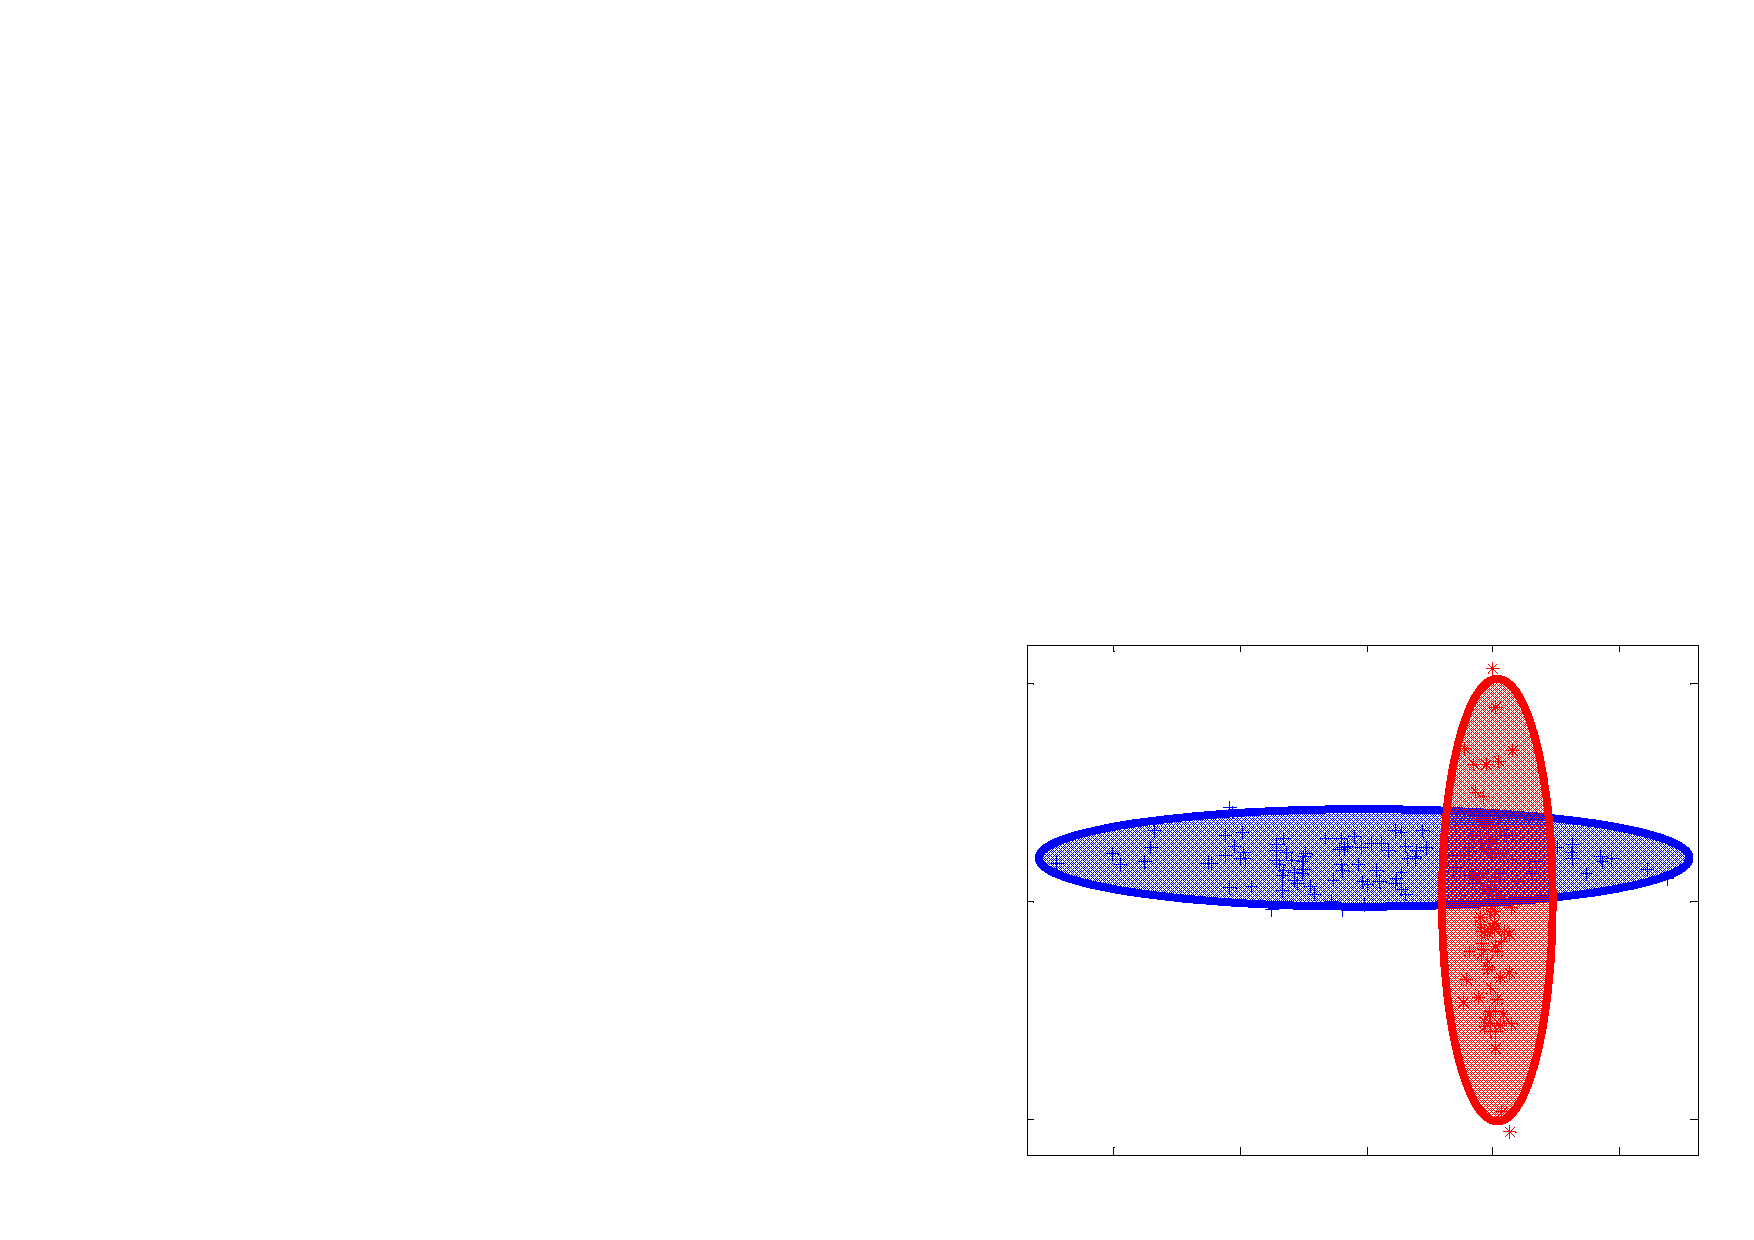
\includegraphics[angle=0,width=1.0\linewidth]{images/unsupervised/gaussian_mixture/gmm_example.pdf}
	%				\caption{Single-Link Dendogram Good K}
				%\label{Enel_QQ_Plot_Normal}
			\end{figure}

		\end{columns}
	%\end{block}

\end{frame}


\ifthenelse{\boolean{highschool}}{

\begin{frame}

	\frametitle{{\color{GradientDescentDiagramOrange}Distribution-based Clustering}: Mixture of Gaussian 1D}

	\begin{block}{Distribuzione gaussiana (o normale o Gauss o Laplace-Gauss)}
%		\begin{itemize}			
			\begin{columns}

				\column{0.37\linewidth}
				$$\mathcal{N}(x\vert\mu, \sigma)= {\frac{1}{\sigma\sqrt{2\pi}}}e^{- {\frac {1}{2}} (\frac {x-\mu}{\sigma})^2}$$
				\begin{scriptsize}
					\begin{itemize}
						\item $\mathcal{N}(\cdot)	=$ densità di probabilità
						\item $\mu =$ media
						\item $\sigma^2 =$ varianza
						\item $\sigma =$	 deviazione standard
					\end{itemize}
					$\qquad$ \underline{\href{https://academo.org/demos/gaussian-distribution/}{Prova con differenti $\mu$ e $\sigma$}}
				\end{scriptsize}

					
				\column{0.63\linewidth}
				\begin{figure}[!htbp]
					\centering
					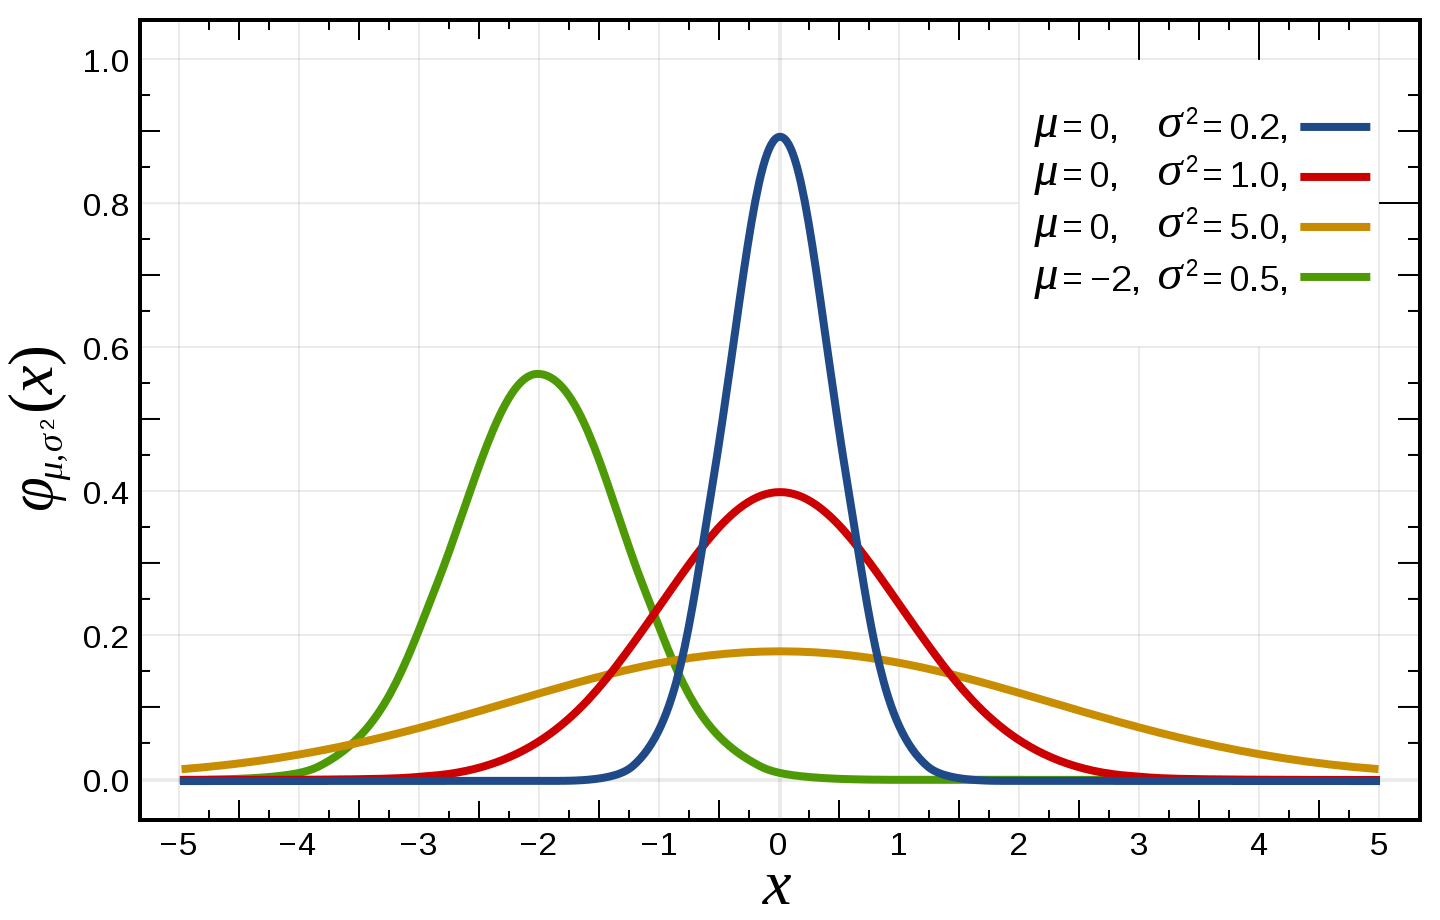
\includegraphics[angle=0,width=1.0\linewidth]{images/unsupervised/gaussian_mixture/gaussian_pdf.png}
		%				\caption{Single-Link Dendogram Good K}
					%\label{Enel_QQ_Plot_Normal}
				\end{figure}
			\end{columns}

%		\end{itemize}
	\end{block}

\end{frame}


\begin{frame}

	\frametitle{{\color{GradientDescentDiagramOrange}Distribution-based Clustering}: Mixture of Gaussian 1D}	

	\begin{block}{Es \#1: un assaggio dell'idea; clusterizzare un dataset con singola feature:}

		\begin{figure}[!htbp]
			\centering
			
			% Foto salvate da una simulazione fatta qui:
			% http://sia.webpopix.org/mixtureModels.html
			\includegraphics<1>[width=0.70\linewidth, height=6.2cm]{images/unsupervised/gaussian_mixture/gmm_idea_0.png}
			\includegraphics<2>[width=0.70\linewidth, height=6.2cm]{images/unsupervised/gaussian_mixture/gmm_idea_1.png}
			\includegraphics<3>[width=0.70\linewidth, height=6.2cm]{images/unsupervised/gaussian_mixture/gmm_idea_2.png}
			\includegraphics<4>[width=0.70\linewidth, height=6.2cm]{images/unsupervised/gaussian_mixture/gmm_idea_3.png}
			%\caption{Single-Link}
			%\label{Enel_HistFit_Normal}
		\end{figure}

	\end{block}

\end{frame}


\begin{frame}

	\frametitle{{\color{GradientDescentDiagramOrange}Distribution-based Clustering}: Mixture of Gaussian 1D}	
	\begin{block}{Es \#2: un assaggio dell'idea; clusterizzare un dataset con singola feature:}
		\centering
		\animategraphics[controls={play, step, stop}, height=5.5cm]{2.0}{images/unsupervised/gaussian_mixture/gmm_1D_K_2/gmm_1D_K_2-}{0}{32}
	\end{block}
		
\end{frame}


\begin{frame}

	\frametitle{{\color{GradientDescentDiagramOrange}Distribution-based Clustering}: Mixture of Gaussian 1D}	
	\begin{block}{Es \#3: un assaggio dell'idea; clusterizzare un dataset con singola feature:}
		\centering
		\animategraphics[controls={play, step, stop}, height=5.5cm]{2.0}{images/unsupervised/gaussian_mixture/gmm_1D_K_3/gmm_1D_K_3-}{0}{41}
	\end{block}
		
\end{frame}


\begin{frame}

	\frametitle{{\color{GradientDescentDiagramOrange}Distribution-based Clustering}: Mixture of Gaussian MultiD}

	\begin{block}{Il passaggio da 1$D$ a 2$D$:}
%		\begin{itemize}
			
			\begin{columns}
				\column{0.45\linewidth}
				\begin{figure}[!htbp]
					\centering
					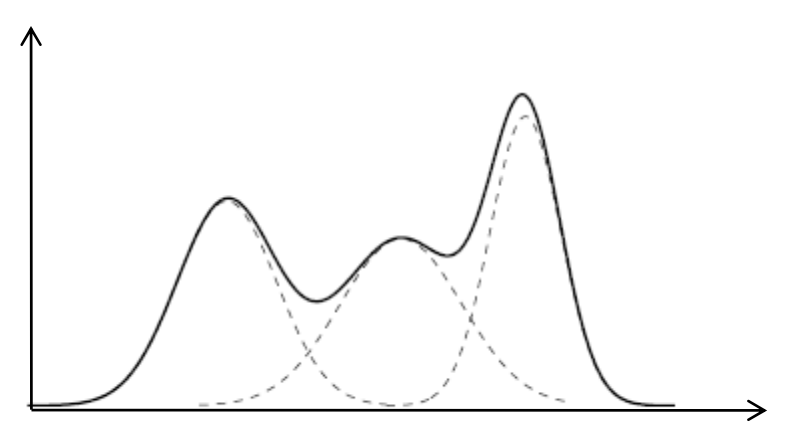
\includegraphics[width=0.85\linewidth]{images/unsupervised/gaussian_mixture/gmm_monovariate.png}
					\caption{GMM applicato su D=1}
				\end{figure}
					
				\column{0.1\linewidth}
				$\rightarrow$
				
				\pause
				
				\column{0.45\linewidth}
				\begin{figure}[!htbp]
					\centering
					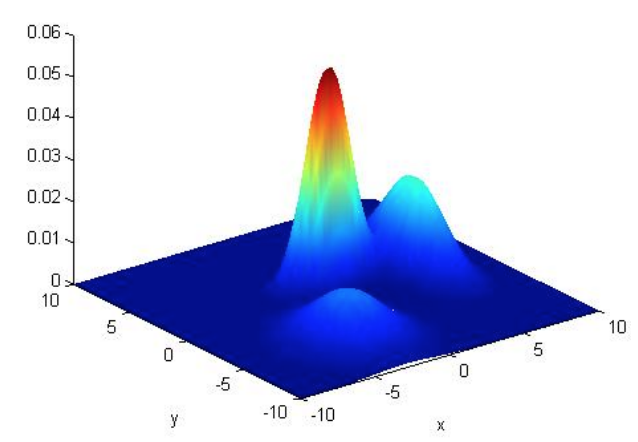
\includegraphics[width=0.85\linewidth]{images/unsupervised/gaussian_mixture/gmm_multivariate.png}
					\caption{GMM applicato su D=2}
				\end{figure}
			\end{columns}
					
%		\end{itemize}
	\end{block}	

\end{frame}


\begin{frame}

	\frametitle{{\color{GradientDescentDiagramOrange}Distribution-based Clustering}: Mixture of Gaussian MultiD}

	\begin{scriptsize}
	\begin{block}{Distribuzione Gaussiana $D = 1$:}
%		\begin{itemize}
			
			\begin{empheq}[box=\fcolorbox{blue!40!black!60}{yellow!10}]{align*}
				\mathcal{N}(x\vert\mu, \sigma)= {\frac{1}{\sigma\sqrt{2\pi}}}e^{- {\frac {1}{2}} (\frac {x-\mu}{\sigma})^2}
			\end{empheq}
			Dove:
			\begin{itemize}
				\item[--] $\mu$ è la media (scalare)
				\item[--] $\sigma$ è la deviazione standard (scalare)
			\end{itemize}
%		\end{itemize}
	\end{block}
	\pause
	\begin{block}{Distribuzione Gaussiana Multivariata $D \geq 1$:}
%		\begin{itemize}
			
			
			\begin{columns}
				\column{0.25\linewidth}
				~
				\column{0.55\linewidth}
				\begin{empheq}[box=\fcolorbox{blue!40!black!60}{yellow!10}]{align*}
					\mathcal{N}(z\vert\mu, C) = (2\pi)^{-\frac{D}{2}} {\vert C\vert}^{-\frac{1}{2}} e^{\frac{-(z-\mu)^T C^{-1} (z-\mu)}{2}}
				\end{empheq}

					
				\column{0.05\linewidth}
				~\\~	\\
				$\rightarrow$
				\column{0.15\linewidth}
				~\\~	\\
				Su R con:  \underline{\href{https://www.rdocumentation.org/packages/LaplacesDemon/versions/16.1.4/topics/dist.Multivariate.Normal}{dmvn}}
			\end{columns}
			
			Dove:
			\begin{itemize}
				\item[--] $z$ è un vettore (vettore colonna $D \times 1$) con le coordinate nello spazio $\mathcal{R}^D$
				\item[--] $\mu$ è il vettore media (vettore colonna $D \times 1$)
				\item[--] $C$ è la matrice di covarianza (matrice $D \times D$)
			\end{itemize}
					
%		\end{itemize}
	\end{block}
	\end{scriptsize}	

\end{frame}



\begin{frame}

	\frametitle{{\color{GradientDescentDiagramOrange}Distribution-based Clustering}: Mixture of Gaussian MultiD}

	\begin{block}{Esempio di normale multivariata con ${\displaystyle {\boldsymbol {\mu }}=\left[{\begin{smallmatrix}0\\0\end{smallmatrix}}\right]}$ and ${\displaystyle {\boldsymbol {\Sigma }}=\left[{\begin{smallmatrix}1&3/5\\3/5&2\end{smallmatrix}}\right]}$}
		\begin{figure}[!htbp]
			\centering
			
			\begin{columns}

				\column{0.5\linewidth}
				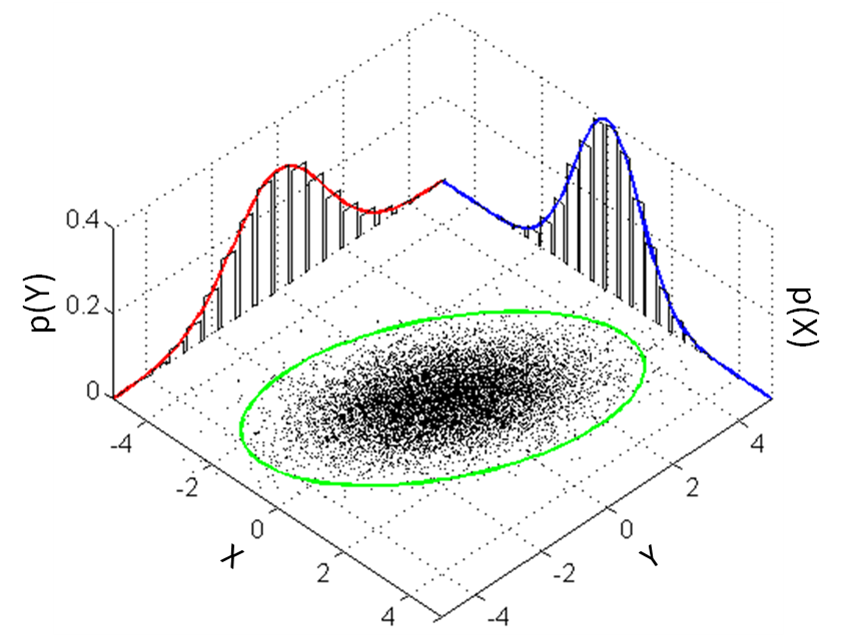
\includegraphics[width=0.8\linewidth]{images/unsupervised/gaussian_mixture/multivariate_normal_1.png}
				\caption{In nero alcuni punti campionati dalla distribuzione, in verde l'ellisse 3-$\sigma$, in blu e rosso le due distribuzioni marginali e i due istogrammi 1-$d$.}
					
				\column{0.5\linewidth}
				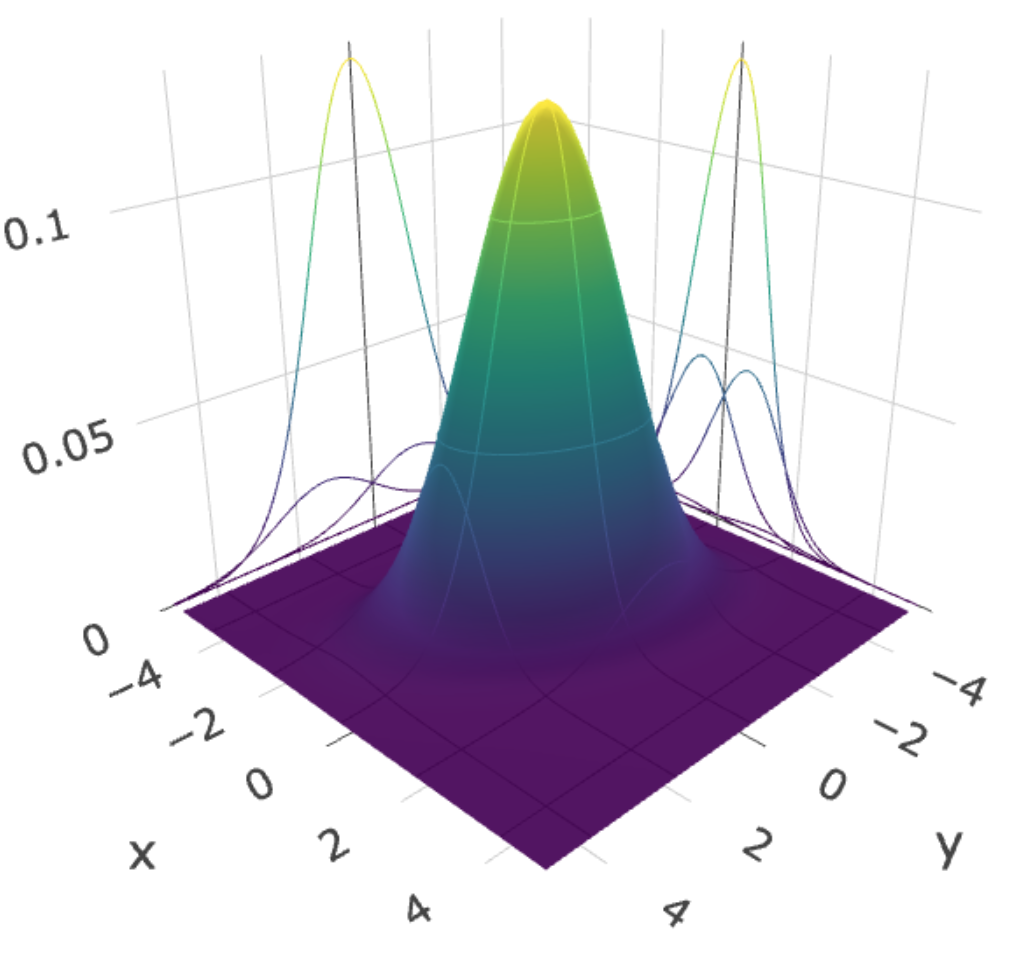
\includegraphics[width=0.85\linewidth]{images/unsupervised/gaussian_mixture/multivariate_normal_2.png}
				\caption{Densità di probabilità.}
			\end{columns}
			
			
		\end{figure}
	\end{block}

\end{frame}

}{}


\begin{frame}

	\frametitle{{\color{GradientDescentDiagramOrange}Distribution-based Clustering}: Mixture of Gaussian}

	%\begin{block}{}
		\begin{itemize}
			\item la densità della distribuzione dei dati in una posizione generica $z$ (vettore colonna) nello spazio delle features $R^D$:
				\begin{empheq}[box=\fcolorbox{blue!40!black!60}{yellow!10}]{align*}
					p(z \vert \Theta )=\sum_{k=1}^{K}\pi_k \mathcal{N}(z\vert\mu_k, C_k)
				\end{empheq}
			\item dove:
				\begin{itemize}
					\item[--] $\Theta = \{ \pi_1, ..., \pi_K, \mu_1, ..., \mu_K, C_1, ..., C_K\}$ è il set dei parametri della mixture di $K$ componenti
					\item[--] $\pi_k$ sono i parametri di mixing per i quali vale:\\
						$\sum\pi_k=1$ e $\pi_k>0$
					\item[--] $\mathcal{N}(z\vert\mu_k, C_k)$ è il valore della $k$-esima Gaussiana multivariata in z:
				\end{itemize}
				
				\begin{empheq}[box=\fcolorbox{blue!40!black!60}{yellow!10}]{align*}
					\mathcal{N}(z\vert\mu_k, C_k) = (2\pi)^{-\frac{D}{2}} {\vert C_k\vert}^{-\frac{1}{2}} e^{\frac{-(z-\mu_k)^T C_{k}^{-1} (z-\mu_k)}{2}}
				\end{empheq}

		\end{itemize}
	%\end{block}

\end{frame}


\begin{frame}

	\frametitle{{\color{GradientDescentDiagramOrange}Distribution-based Clustering}: Mixture of Gaussian}

	%\begin{block}{}
		\begin{empheq}[box=\fcolorbox{blue!40!black!60}{yellow!10}]{align*}
			p(z \vert \Theta )=\sum_{k=1}^{K}\pi_k \mathcal{N}(z\vert\mu_k, C_k)
		\end{empheq}

		\begin{itemize}
			\item i parametri da stimare sono:
				\begin{itemize}
					\item[--] il numero $K$ di clusters
					\item[--] i parametri di mixing $\pi_1,...,\pi_K$ (valori scalari)
					\item[--] i vettori delle medie $\mu_1,...,\mu_K$ (vettori colonna)
					\item[--] le matrici di covarianza $C_1,...,C_K$
				\end{itemize}
			\item rispetto a K-mean, il numero di parametri è maggiore. Pertanto, dovrebbe essere disponibile un numero maggiore di dati
				\begin{itemize}
					\item[--] altrimenti, è molto probabile che si otterrà una stima imprecisa dei valori dei parametri
				\end{itemize}

		\end{itemize}
	%\end{block}

\end{frame}


\begin{frame}

	\frametitle{{\color{GradientDescentDiagramOrange}Distribution-based Clustering}: Gaussian Mixture (GM)}

	%\begin{block}{}


		\begin{itemize}
			\item tipicamente, si presume che il numero $K$ di componenti gaussiane sia noto
			\item i valori degli altri parametri sono stimati tramite l'algoritmo \textbf{Expectation-Maximization}
			\item si tratta di una procedura che aggiorna iterativamente i valori dei parametri attraverso la definizione di una \textbf{hidden ownership variable} $x_{ik}$ (valore scalare):
				\begin{itemize}
					\item[--] $x_{ik}$ rappresenta la probabilità (likelihood) che l'$i$-esimo dato sia generato dal $k$-esimo componente della mixture di gaussiane
				\end{itemize}

		\end{itemize}
	%\end{block}

\end{frame}


\begin{frame}

	\frametitle{{\color{GradientDescentDiagramOrange}Distribution-based Clustering}: EM algorithm for GM}

	%\begin{block}{}
		\begin{enumerate}
			\item inizializzazione randomica dei parametri $\pi_k, \mu_k, C_k$
			\item (\textbf{E}) calcola la \textbf{expectation} delle \textit{ownership variables} $x_{ik}$:
				\begin{scriptsize}
					\begin{empheq}[box=\fcolorbox{blue!40!black!60}{yellow!10}]{align*}
						x_{ik} = \frac{\pi_k \mathcal{N}(z_i\vert\mu_k,C_k)}{\sum_{j=1}^{K}\pi_j \mathcal{N}(z_i\vert\mu_j,C_j)} \qquad \left( \implies \sum_{k=1}^{K}x_{ik} = 1 \right)
					\end{empheq}
				\end{scriptsize}
			\item (\textbf{M}) utilizza le expectation delle \textit{ownership variables} per effettuare una stima della \textbf{massima verosimiglianza} dei parametri $\pi_k, \mu_k, C_k$:
				\begin{scriptsize}
					\begin{empheq}[box=\fcolorbox{blue!40!black!60}{yellow!10}]{align*}
						\pi_k = \frac{1}{N} \sum_{i=1}^{N}x_{ik} \qquad \mu_k = \frac{1}{N\pi_k}\sum_{i=1}^{N}x_{ik}z_i \qquad C_k = \frac{1}{N\pi_k} \sum_{i=1}^{N} x_{ik} (z_i-\mu_k)(z_i-\mu_k)^T
					\end{empheq}
				\end{scriptsize}
			\item Interrompi se la \textbf{log-likelihood} non è cambiata in modo significativo rispetto alla configurazione dell'iterazione precedente (vedi dopo lg-$\ell$).\\
				Altrimenti vai al passaggio 2.
		\end{enumerate}

	%\end{block}

\end{frame}


\begin{frame}

	\frametitle{{\color{GradientDescentDiagramOrange}Distribution-based Clustering}: EM algorithm for GM}

	%\begin{block}{}
		\begin{figure}[!htbp]
			\centering
			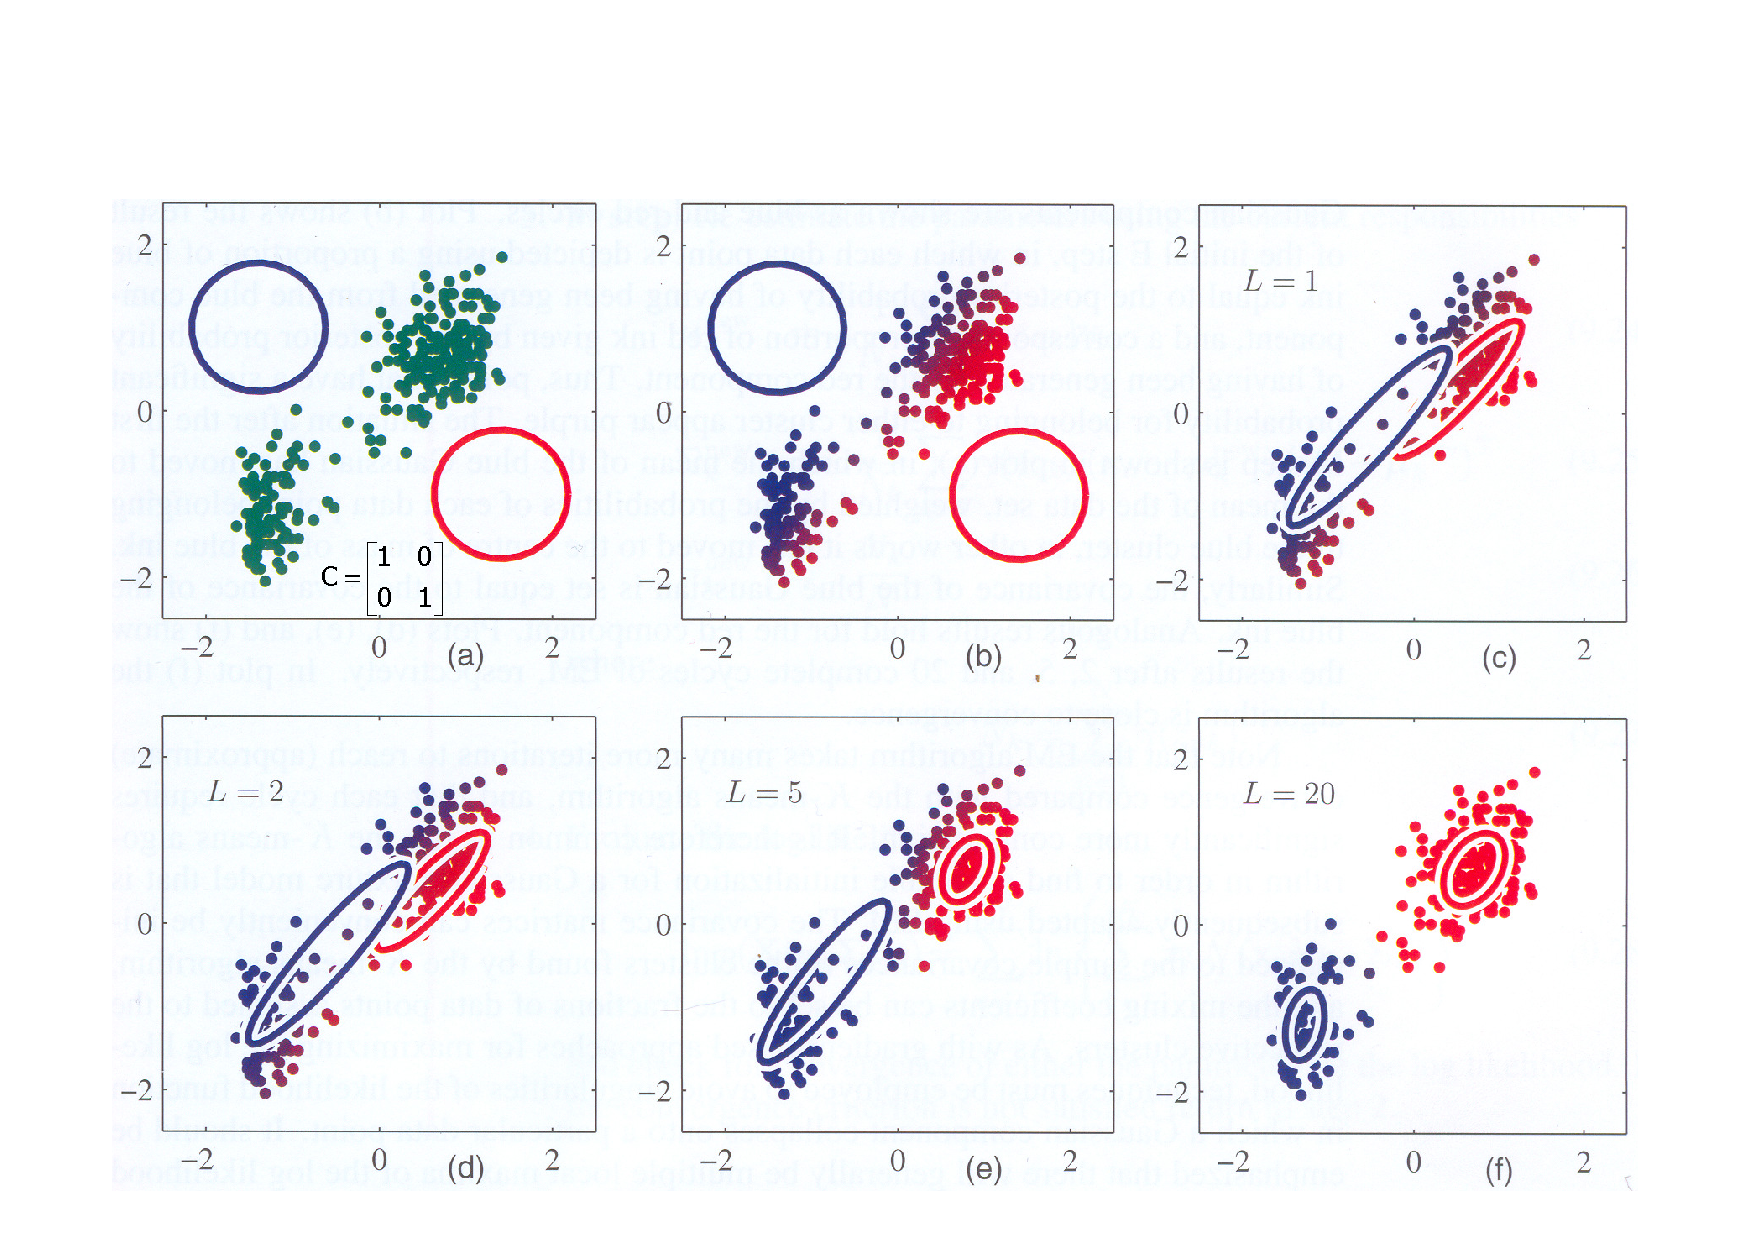
\includegraphics[width=0.9\linewidth]{images/unsupervised/gaussian_mixture/gmm_1.pdf}
					%\caption{Stripe Radar for Fraud Detection}
		\end{figure}
	%\end{block}

\end{frame}


\begin{frame}

	\frametitle{{\color{GradientDescentDiagramOrange}Distribution-based Clustering}: EM algorithm for GM}

		La convergenza viene generalmente rilevata calcolando il valore della \textbf{log-likelihood} dopo ogni iterazione e interrompendosi quando sembra non cambiare in modo significativo da un'iterazione alla successiva.\\
		Si noti che la log-likelihood (nell'ipotesi IID) è definita come segue:
		\begin{empheq}[box=\fcolorbox{blue!40!black!60}{yellow!10}]{align*}
			log\text{ }\ell (\Theta) = \sum_{i=1}^{N} log\text{ }p(z_i \vert \Theta) = \sum_{i=1}^{N} \left( log \sum_{k=1}^{K} \pi_k \mathcal{N}(z_i\vert\mu_k,C_k) \right)
		\end{empheq}

		Dove:
		\begin{itemize}
			\item[--] $z_i$ è la $i$-esima istanza del dataset
			\item[--] $K$ è il numero di clusters
			\item[--] $\pi_1,...,\pi_K$ sono i parametri di mixing (valori scalari)
			\item[--] $\mu_1,...,\mu_K$ sono i vettori delle medie (vettori colonna)
			\item[--] $C_1,...,C_K$ sono le matrici di covarianza 
		\end{itemize}
		
\end{frame}


\begin{frame}

	\frametitle{{\color{GradientDescentDiagramOrange}Distribution-based Clustering}: EM algorithm for GM}	\centering
		\animategraphics[controls={play, step, stop}, height=7cm]{7.0}{images/unsupervised/gaussian_mixture/em_for_gm/em_for_gm-}{0}{49}
\end{frame}


\begin{frame}

	\frametitle{{\color{GradientDescentDiagramOrange}Distribution-based Clustering}: EM algorithm for GM}
	%\begin{block}{}
		\begin{figure}[!htbp]
			\centering
			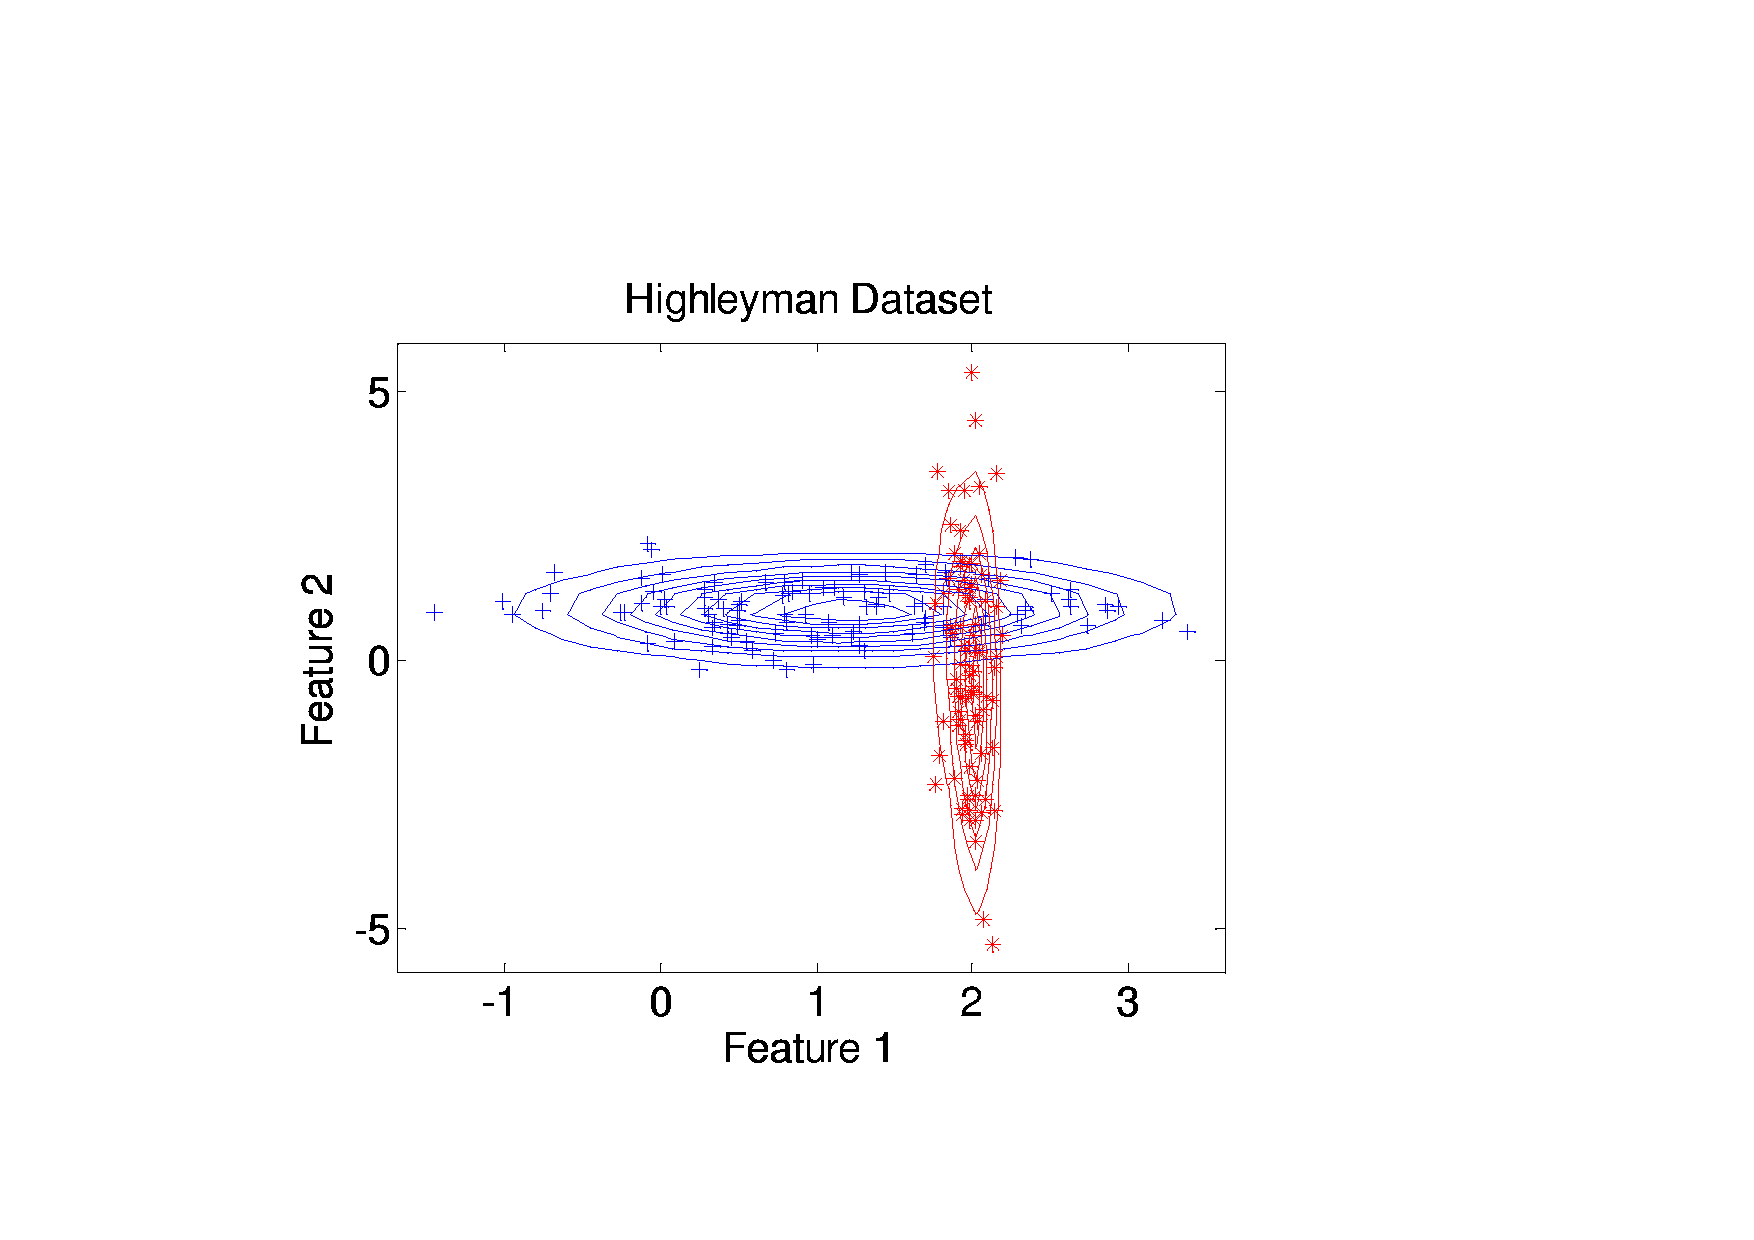
\includegraphics[width=0.6\linewidth]{images/unsupervised/gaussian_mixture/gmm_2.pdf}
					%\caption{Stripe Radar for Fraud Detection}
		\end{figure}
	%\end{block}

\end{frame}


\begin{frame}

	\frametitle{{\color{GradientDescentDiagramOrange}Distribution-based Clustering}: EM algorithm for GM}

	%\begin{block}{}
		\begin{itemize}
			\item la stima dei valori dei parametri potrebbe non essere accurata se il numero dei punti del dataset è basso
		\end{itemize}
		\begin{figure}[!htbp]
			\centering
			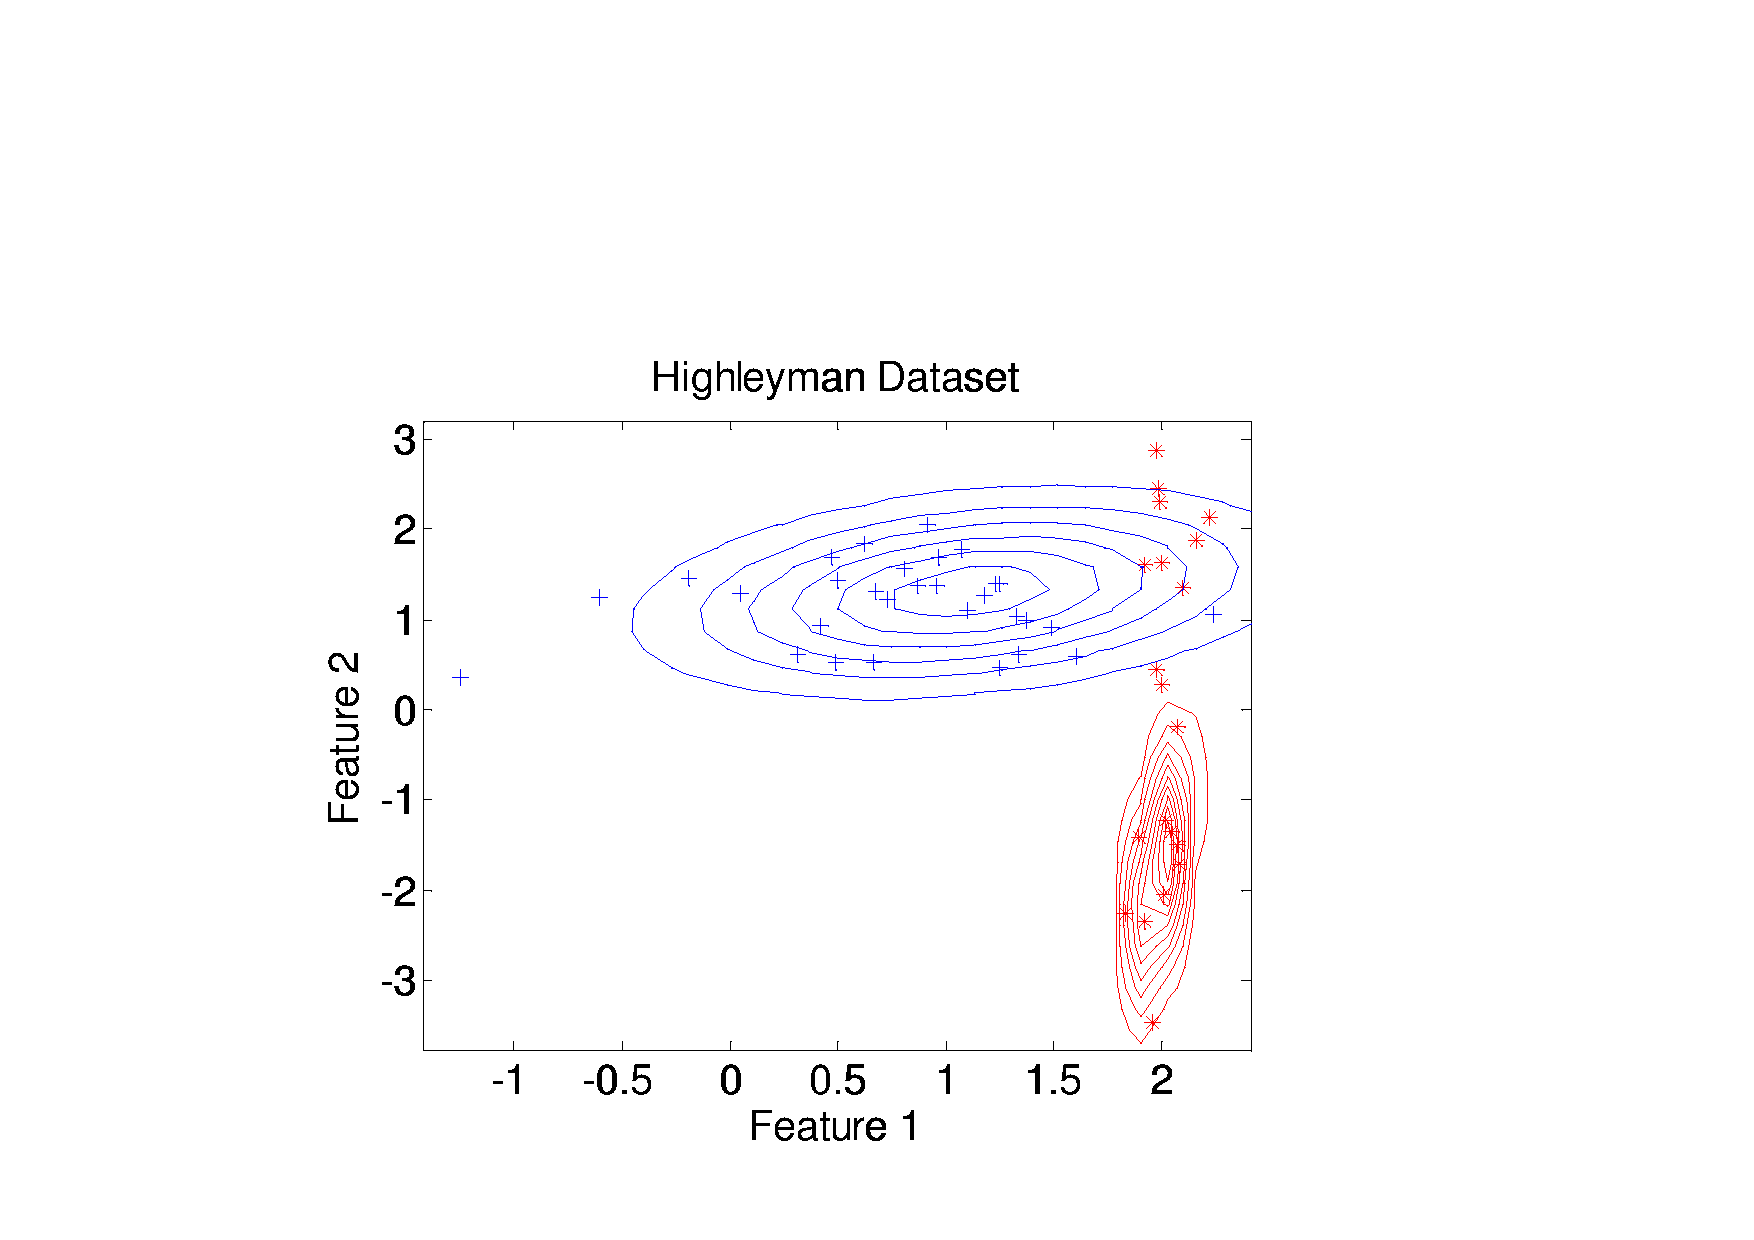
\includegraphics[width=0.6\linewidth]{images/unsupervised/gaussian_mixture/gmm_3.pdf}
					%\caption{Stripe Radar for Fraud Detection}
		\end{figure}
	%\end{block}

\end{frame}


\begin{frame}

	\frametitle{{\color{GradientDescentDiagramOrange}Distribution-based Clustering}: EM algorithm for GM}

	%\begin{block}{}
		\begin{itemize}
			\item Una volta determinati i parametri della mistura gaussiana, la segmentazione si ottiene assegnando l'$i$-esima istanza al cluster con il valore massimo della \textit{ownership variable} $x_{ik}$:
			\begin{empheq}[box=\fcolorbox{blue!40!black!60}{yellow!10}]{align*}
				x_{ik} = \frac{\pi_k \mathcal{N}(z_i\vert\mu_k,C_k)}{\sum_{j=1}^{K}\pi_j \mathcal{N}(z_i\vert\mu_j,C_j)}
			\end{empheq}
		\end{itemize}
	%\end{block}

\end{frame}


\begin{frame}

	\frametitle{{\color{GradientDescentDiagramOrange}Distribution-based Clustering}: segmentazione con il GMM}

%	\begin{block}{K-means: considerazioni}
		\begin{figure}[!htbp]
				\centering
				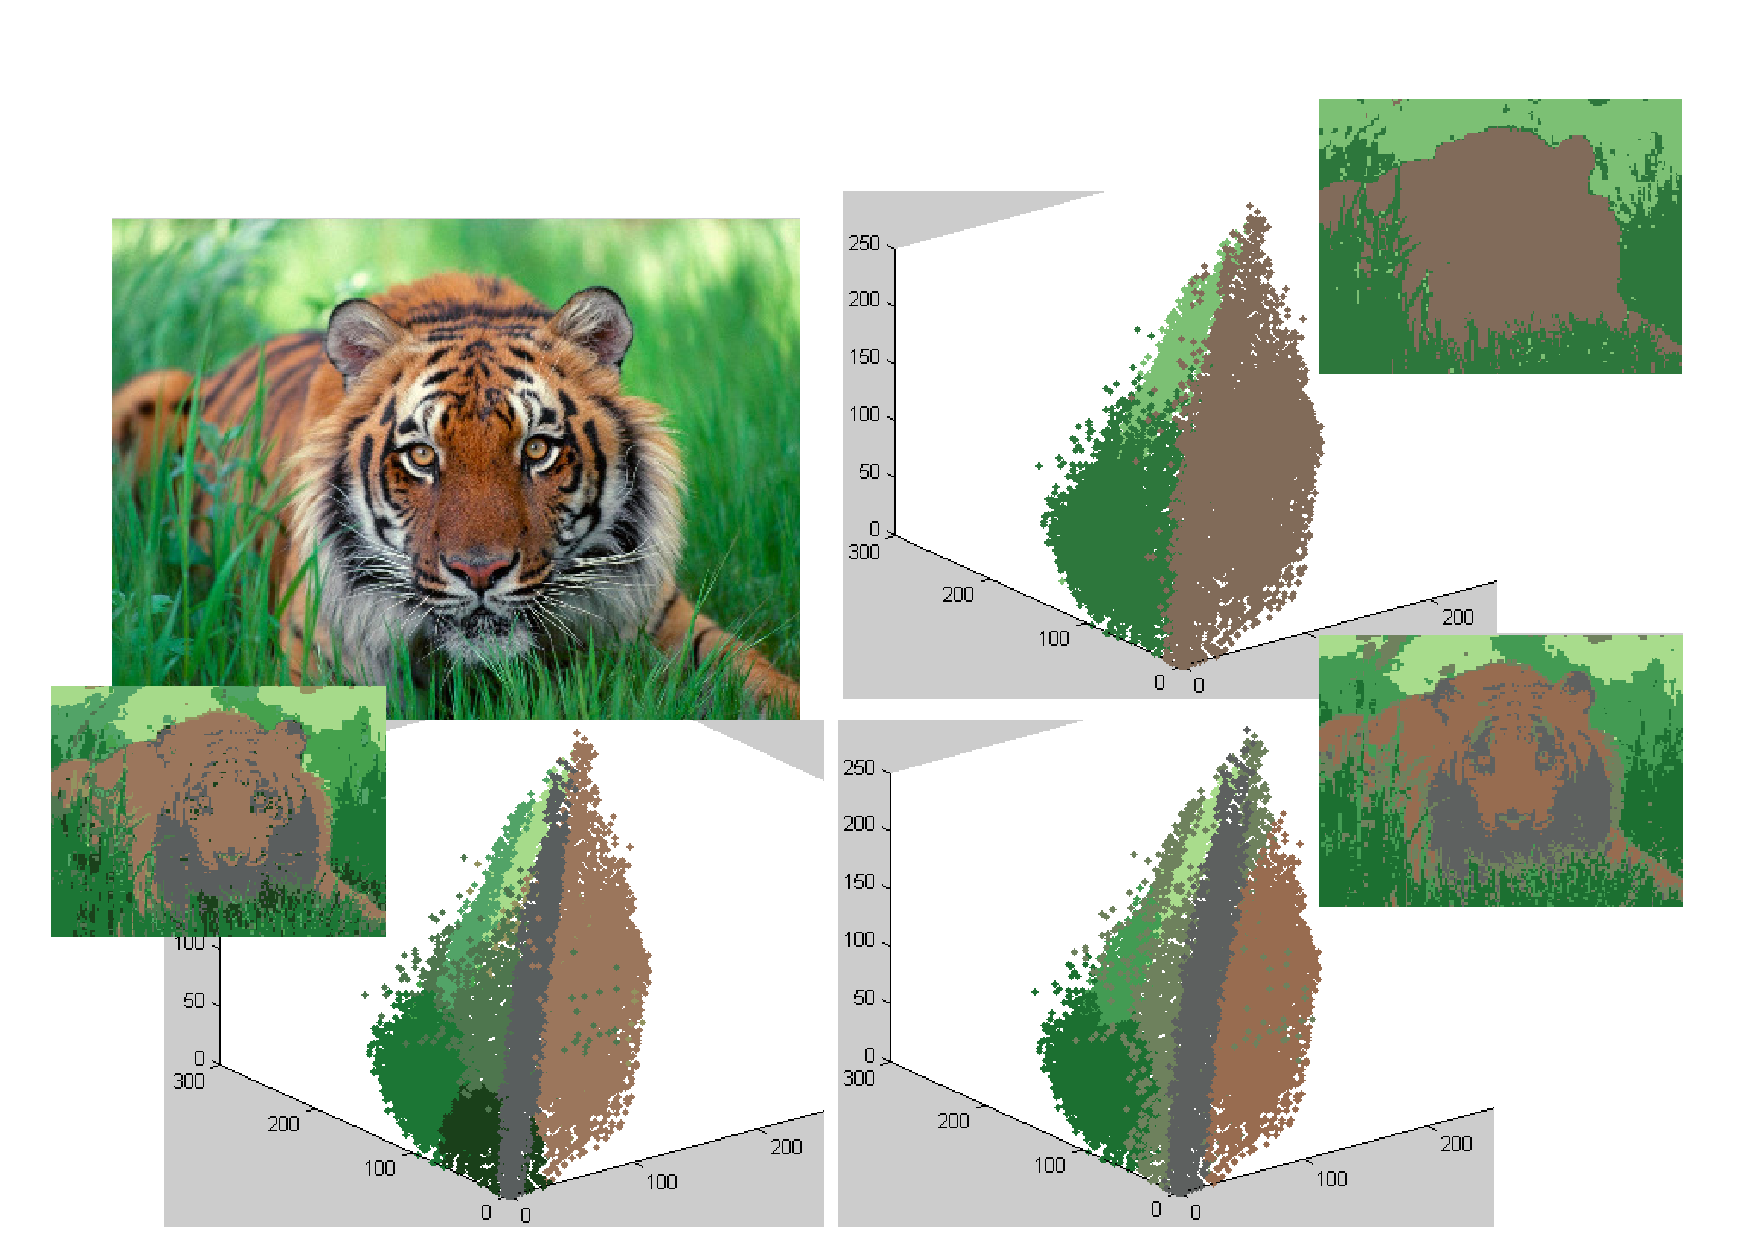
\includegraphics[angle=0,width=0.85\linewidth]{images/unsupervised/gaussian_mixture/gmm_lion.pdf}
%				\caption{Single-Link Dendogram Good K}
				%\label{Enel_QQ_Plot_Normal}
			\end{figure}
%	\end{block}

\end{frame}


\begin{frame}

	\frametitle{{\color{GradientDescentDiagramOrange}Distribution-based Clustering}: segmentazione con il GMM}

%	\begin{block}{K-means: considerazioni}
		\begin{figure}[!htbp]
				\centering
				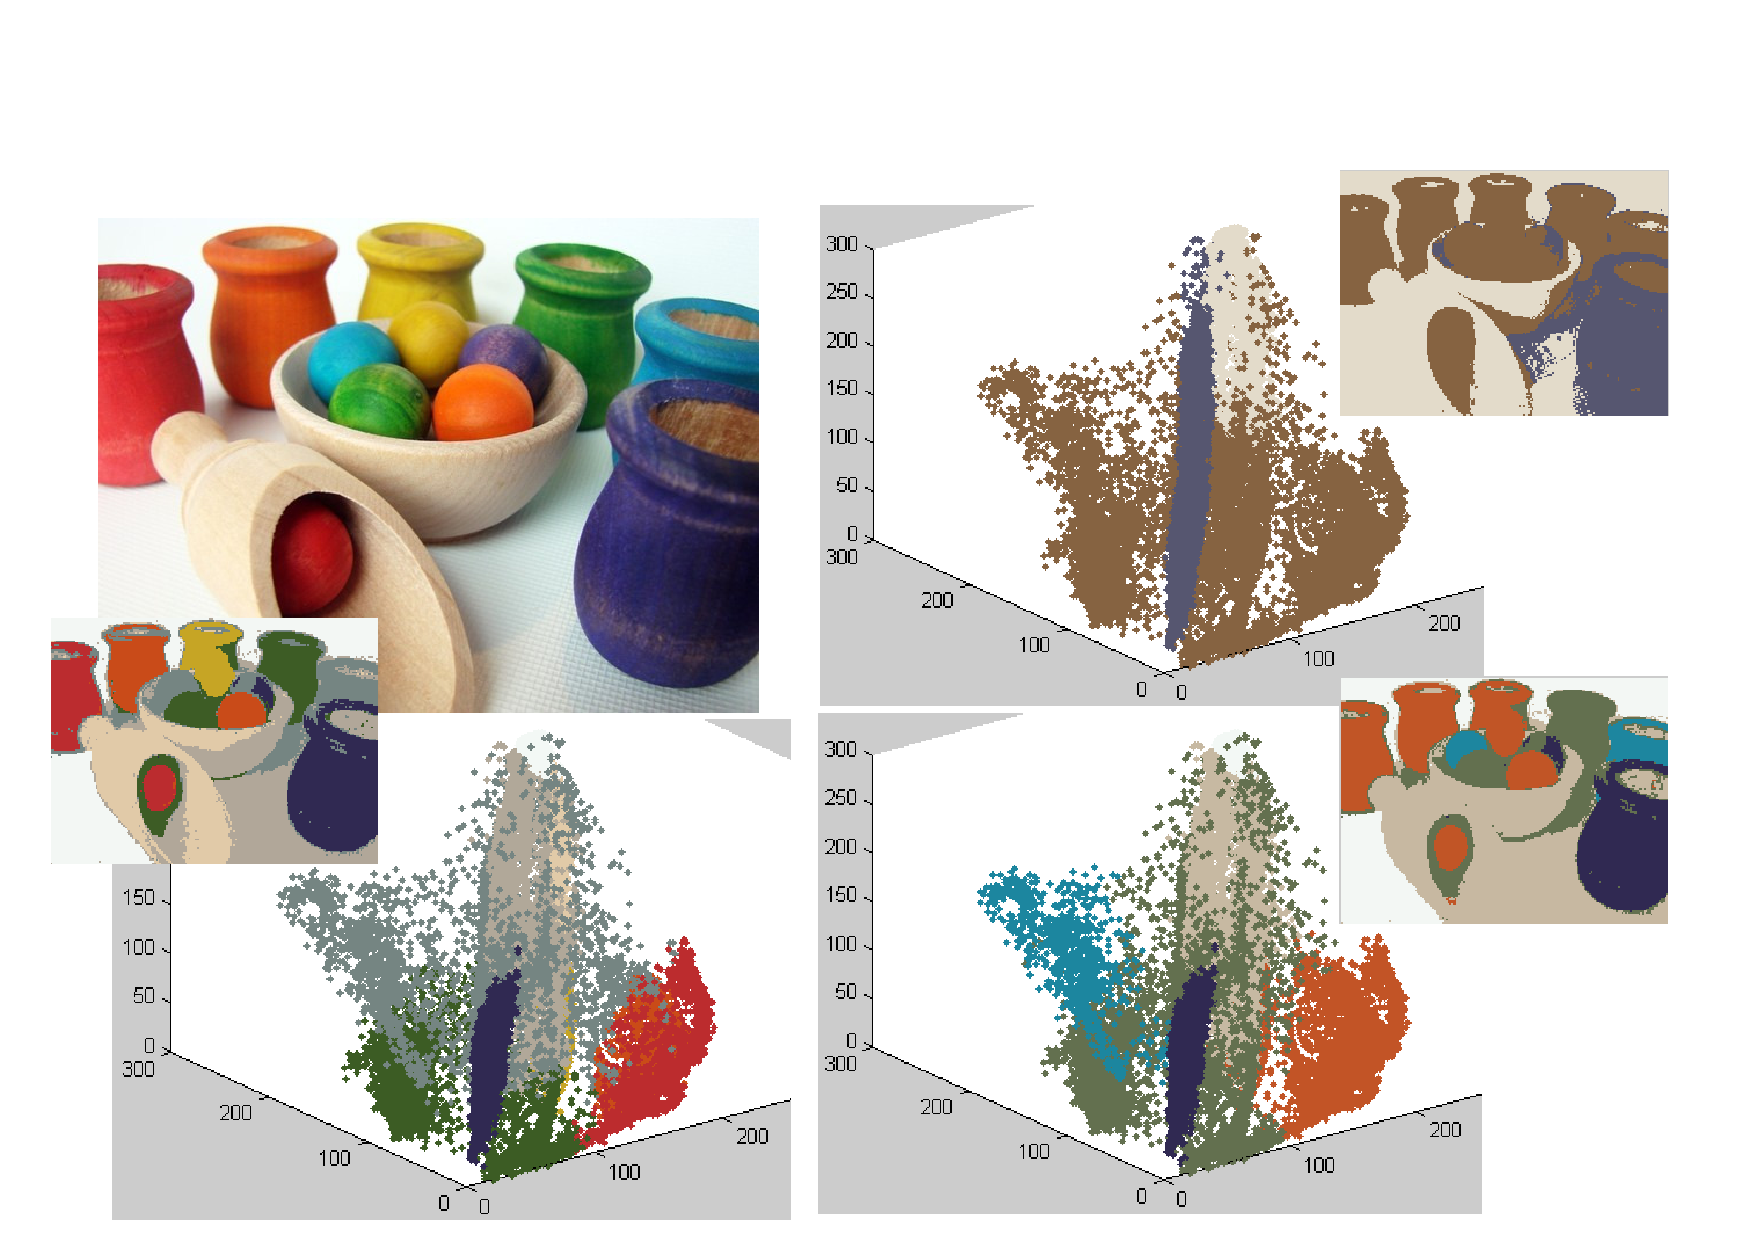
\includegraphics[angle=0,width=0.9\linewidth]{images/unsupervised/gaussian_mixture/gmm_pots.pdf}
%				\caption{Single-Link Dendogram Good K}
				%\label{Enel_QQ_Plot_Normal}
			\end{figure}
%	\end{block}

\end{frame}


\begin{frame}

	\frametitle{{\color{GradientDescentDiagramOrange}Distribution-based Clustering}: limiti del GMM}

%	\begin{block}{K-means: considerazioni}
		\begin{itemize}
			\item inizializzazioni con parametri diversi può portare a differenti risultati
				\begin{itemize}
					\item[--] in effetti, la procedura iterativa per la stima dei parametri può fermarsi in minimi locali della funzione obiettivo
				\end{itemize}
			\item  il numero di componenti della mistura deve essere scelto in partenza
			\item poiché devono essere stimati molti parametri, è richiesto un dataset molto ampio rispetto a quanto necessario con K-means
			\item nessuna garanzia generale che la distribuzione dei dati all'interno di ciascun cluster sia gaussiana
		\end{itemize}
%	\end{block}

\end{frame}


\begin{frame}

	\frametitle{{\color{GradientDescentDiagramOrange}Distribution-based Clustering}: confronto con altre tecniche}

%	\begin{block}{K-means: considerazioni}
		\begin{figure}[!htbp]
				\centering
				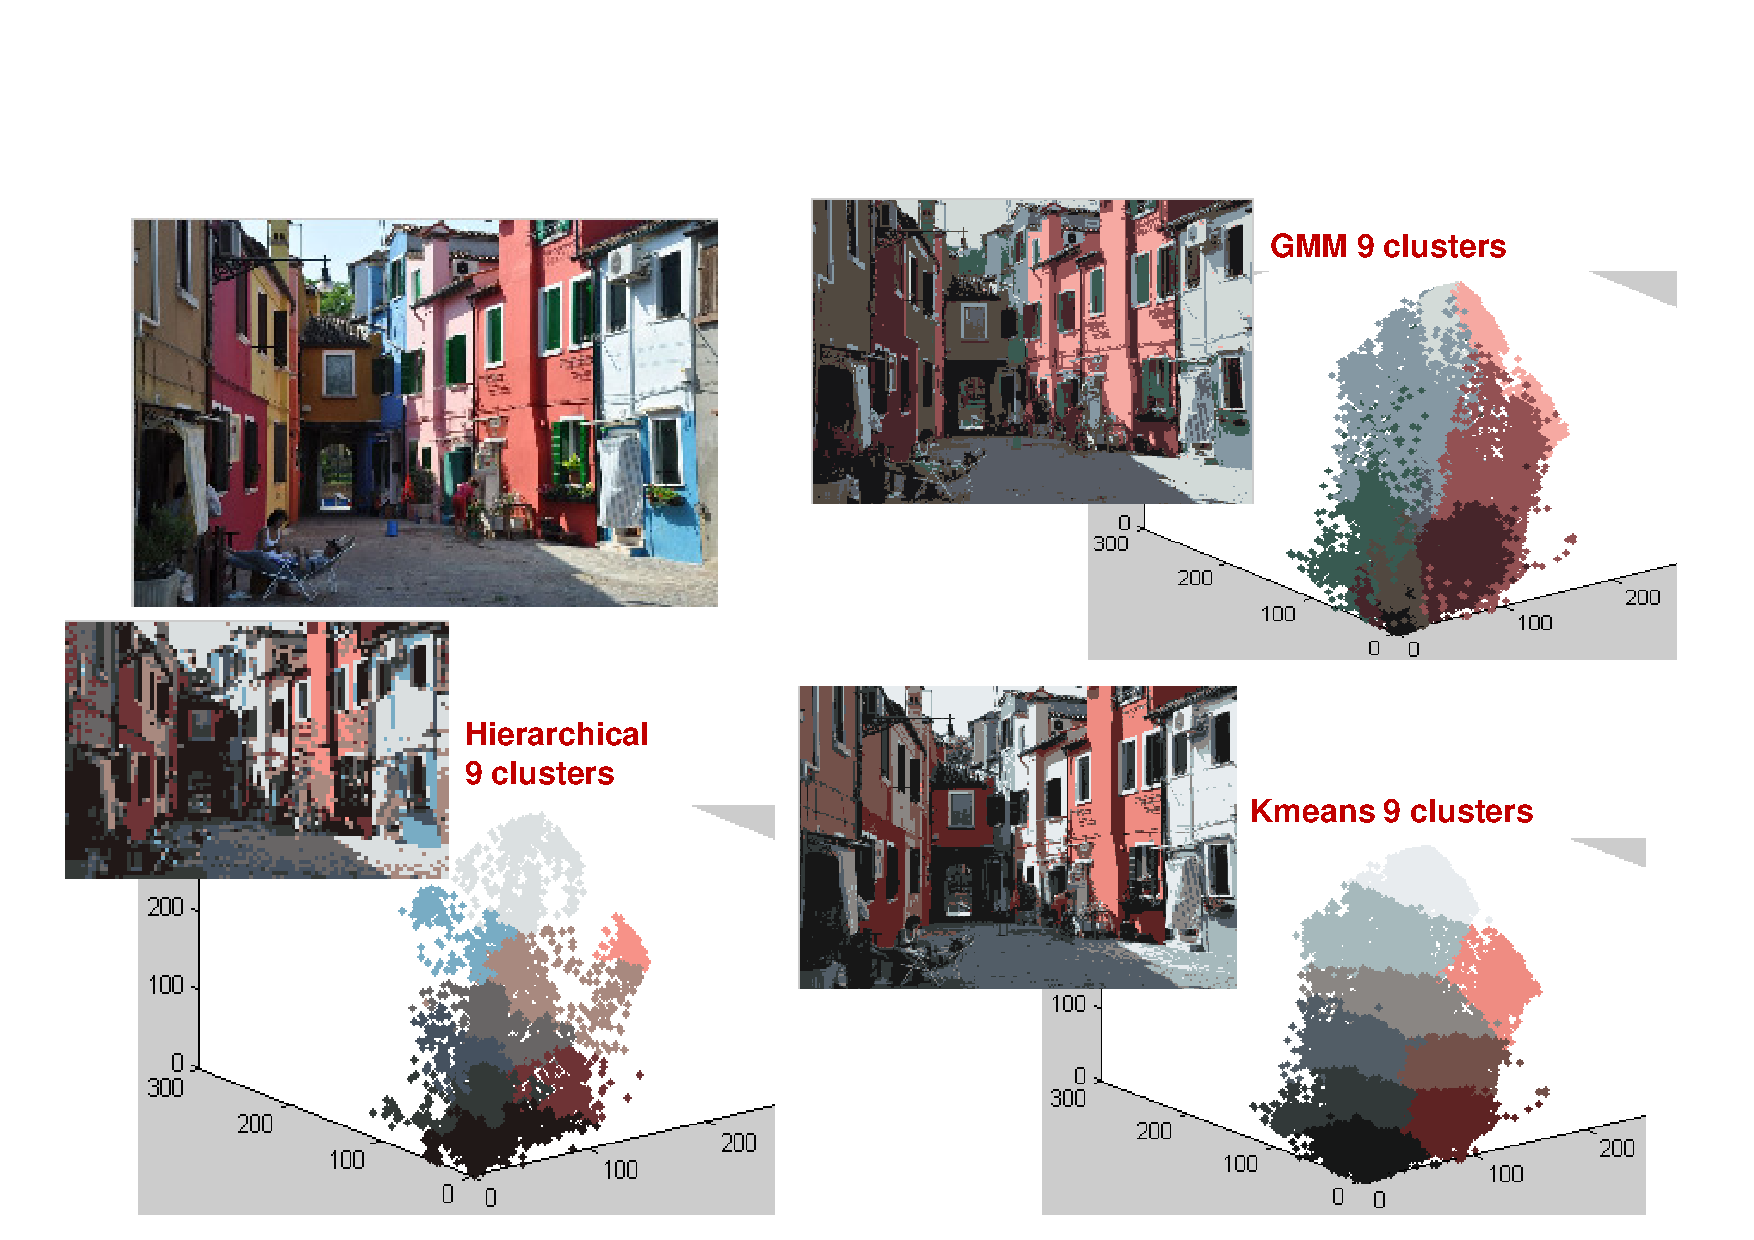
\includegraphics[angle=0,width=0.9\linewidth]{images/unsupervised/gaussian_mixture/hierarchical_vs_kmeans_vs_gmm.pdf}
%				\caption{Single-Link Dendogram Good K}
				%\label{Enel_QQ_Plot_Normal}
			\end{figure}
%	\end{block}

\end{frame}
